%%%%%%%%%%%%%%%%%%%%%%%%%%%%%%%%%%%%%%%%%%%%%%%%%%%%%%%%%%%%%%%%%%%%%%%%%%%%%%%%
% \chapter[Wind Farm Cabling Problem]{Wind Farm Cabling Problem\footnote{This
% chapter is partly published in~\parencite{Leh17,Weg17}.}}
% 
\Chapter{Transmission Network Expansion Planning}{The Wind Farm
Cabling Problem -- A Greenfield Approach}{
\footnote{This chapter is partly published in~\parencite{Leh17,Weg17}.}}
% 
\label{ch:wfcp}
\glsresetall
%%%%%%%%%%%%%%%%%%%%%%%%%%%%%%%%%%%%%%%%%%%%%%%%%%%%%%%%%%%%%%%%%%%%%%%%%%%%%%%%
% 
Sustainability is an important aspect of the goal of improving and preserving
the existence of human society. Accordingly, renewable energy sources play an
important role. The renewable energy act~\acrshort{eeg}~2017 aims for~40\%
to~45\% of electricity to be produced from renewable energy producers to gross
electricity consumption until~2025 and~55\% to~60\%
until~2035~\parencite{online:juris-eeg2017-zweck-und-ziel-des-gesetzes}. Thus,
it is expected that the current trend of adding renewable energy producers, will
continue~\parencite{online:eeg2014,
online:iwr-offshore-windindustrie-future-europe-data, 969970}.

Wind farms transform wind energy into electrical energy and present an important
and one of the most promising renewable energy producers (\cref{ch:intro}) for
today's and future power grid. In contrast to traditional power plants, which
produce the power in a centralized way
(see~\cref{ch:intro:fig:power-grid-structure} on
Page~\pageref{ch:intro:fig:power-grid-structure}), wind farms aggregate the
power of multiple wind turbines, each injecting power at around~$33$~\gls{kv}
(medium voltage level), \eg, the Hornsea Project One offshore wind farm is
planned to have up to~$240$ turbines~\parencite{online:hornsea-project-one}. As
the number of wind turbines increases, algorithms for planning a wind farm
cabling have to handle this amount of wind turbines. If we consider for instance
a wind turbine of~$3.6$~\gls{mw} then the number of wind turbines increases
worldwide from 2014 to 2015 by~$38$\%
(see~\cref{ch:wfcp:tbl:windfarm-world-statistic}). The biggest planned offshore
wind farm so far with approximately~$300$ turbines is the Hornsea Project
Three~\parencite{online:hornsea-project-three}. In total, the European grid has
3\,344 connected turbines on 82 offshore wind
farms~\parencite{online:wind-europe-key-trend-H1-2016}. The onshore wind farms
Terra-Gen with 617 turbines and Gansu with more than~$3\,500$ turbines represent
two of the largest onshore wind farm projects in North America and China,
respectively.
% 
\Cref{ch:wfcp:tbl:windfarm-world-statistic} shows that the annual potential of
offshore power production compared to the current annual electricity consumption
worldwide is about~$80$\% larger~\parencite{969970}. Thus, satisfying a
reasonable portion of the annual consumption of electricity with wind energy
seems to be possible and reducing the cabling costs is important to reduce the
trade-off between usage and expenses for wind farms~\parencite{4523827}.
% 
Since it is expected that the trend of adding renewable energy sources, such as
wind turbines, will continue and accelerate~\parencite{online:eeg2014,
online:iwr-offshore-windindustrie-future-europe-data, 969970}, the number of
wind turbines and wind farms will increase. This gives an indicator for
realistic instance sizes.

In this chapter, we focus on network planning for wind farms due to a high
potential of cost savings~\parencite{5427895} and a rapidly increasing number of
planned projects~\parencite{online:offshore-windfarm-db,
online:iwr-offshore-windindustrie-future-europe-data}.
% 
The design process of a wind farm includes a variety of decisions that influence
the construction and operation costs~\cite{doi:10.1080/09398368.2006.11463608}.
Typical layout and design factors are presented in~\cite{5275322} such as the
turbine locations, terrain, landowner requirements, and wind profiles, to name a
few. A large fraction of the investment is needed for the cables, cable laying
and substations~\cite{5427895}. Thus, reducing the cabling costs reduces the
trade-off between usage and expenses of wind farms~\cite{4523827}. We focus on
network planning for wind farms due to a high potential of cost
savings~\cite{5427895} and an increasing number of planned
projects~\cite{online:offshore-windfarm-db,
online:iwr-offshore-windindustrie-future-europe-data}.
% 
\begin{table}[t!]
    \centering
    % 
    \caption[Installed offshore wind farm power]{The roughly installed offshore
    wind power (status February
    2016)\parencite{online:iwr-offshore-windindustrie-current-world-data,
    online:iwr-offshore-windindustrie-future-europe-data} increases
    significantly from 2014 to 2015. The number of
    turbines~$\fmagnitude{\glssymbol{generators}}$ is based on the total power
    and assumes that all wind turbines have a power rating
    of~\SI{3.6}{\gls{mw}}, which matches today's dominating Siemens SWT-3.6
    turbines. In the last three columns the annual consumption of electricity
    (El. Cons.) and total energy consumption (Tot. E.) is compared to the
    potential offshore wind energy (Max. Pot.), respectively~\parencite{Gar93,
    online:Enerdata2016}.}
    % 
    \label{ch:wfcp:tbl:windfarm-world-statistic}
    % 
    \setlength{\tabcolsep}{1.5ex}
    % 
    % latex table generated in R 3.2.2 by xtable 1.8-0 package
% Wed Jan 27 11:17:04 2016
% {\setlength{\tabcolsep}{0.0em}}
% \setlength{\tabcolsep}{-2pt}   % set length to -2pt
\addtolength{\tabcolsep}{-0.5pt} % reduce space by -2pt
{\renewcommand{\arraystretch}{2}}% for the vertical padding
% 
% \small
%
\begin{tabular}{%
  l>{\centering\arraybackslash}%
  % 
  r>{\centering\arraybackslash}%
  r>{\centering\arraybackslash}%
  % 
  r>{\centering\arraybackslash}%
  r>{\centering\arraybackslash}%
  % 
  r>{\centering\arraybackslash}%
  r>{\centering\arraybackslash}%
  % 
  r%
}%
%-------------------------------------------------------------------------------
\toprule
%-------------------------------------------------------------------------------
& \multicolumn{2}{c}{2015}
& \multicolumn{2}{c}{2014}
& \multicolumn{2}{c}{2015}  
& \multicolumn{1}{c}{---}
\\
%-------------------------------------------------------------------------------
%-------------------------------------------------------------------------------
&
&
%
&
&
%
& \multicolumn{1}{c}{El. Cons.}
& \multicolumn{1}{c}{Tot. E.}	
%
& \multicolumn{1}{c}{Max. Pot.}
\\
%-------------------------------------------------------------------------------
%-------------------------------------------------------------------------------
\cmidrule(lr){2-3}\cmidrule(lr){4-5}\cmidrule(lr){6-7}\cmidrule(lr){8-8}  
& in \SI{}{\MW}
& $\fmagnitude{\glssymbol{generators}}$ 
%
& in \SI{}{\MW} 
& $\fmagnitude{\glssymbol{generators}}$ 
%
& \multicolumn{1}{c}{in~\SI{}{\tera\watt\hour\per\year}} 
& \multicolumn{1}{c}{in~\SI{}{\tera\watt\hour\per\year}}
% 
& \multicolumn{1}{c}{in~\SI{}{\tera\watt\hour\per\year}} 
\\
%-------------------------------------------------------------------------------
%-------------------------------------------------------------------------------
 \midrule  
%-------------------------------------------------------------------------------
%-------------------------------------------------------------------------------
\rowcolor{Table-Line-Marker}
\textbf{World}%
& \SI{12100}{}%
& \SI{3362}{}%
& \SI{8800}{}%
& \SI{2444}{}%
& \SI{20568}{}%
& \SI{160240}{}%
& \SI{36990}{}%
\\ 
%-------------------------------------------------------------------------------
\textbf{Europe}%
& \SI{11000}{}%
& \SI{3056}{}%
& \SI{8050}{}%
& \SI{2237}{}%
& \SI{3291}{}%
& \SI{20930}{}%
& \SI{8480}{}%
\\
%------------------------------------------------------------------------------- 
\rowcolor{Table-Line-Marker}
\hspace{2mm}UK%
& \SI{5100}{}%
& \SI{1417}{}%
& \SI{4500}{}%
& \SI{1250}{}%
& \SI{312}{}%
& \SI{2080}{}%
& \SI{986}{}%
\\
%------------------------------------------------------------------------------- 
\hspace{2mm}Germany%
& \SI{3300}{}%
& \SI{917}{}%
& \SI{1050}{}%
& \SI{292}{}%
& \SI{521}{}%
& \SI{3550}{}%
& \SI{237}{}%
\\%
%-------------------------------------------------------------------------------
\rowcolor{Table-Line-Marker}
\hspace{2mm}Denmark	
& \SI{1300}{}
& \SI{362}{}
& \SI{1300}{} 	
& \SI{362}{}
& ---
& ---
& \SI{550}{}%
\\%
%-------------------------------------------------------------------------------
\textbf{North}
& 
& 
& 
& 
& 
& 
&
\\%
%-------------------------------------------------------------------------------
  \multirow[b]{-2}{*}{\textbf{America}}
& \multirow[c]{-2}{*}{\SI{0}{}}%
& \multirow[c]{-2}{*}{---}%
& \multirow[c]{-2}{*}{\SI{0}{}}%
& \multirow[c]{-2}{*}{---}%
& \multirow[c]{-2}{*}{\SI{4342}{}}%
& \multirow[c]{-2}{*}{\SI{28450}{}}%
& \multirow[c]{-2}{*}{\SI{9860}{}}%
\\%
%-------------------------------------------------------------------------------
\rowcolor{Table-Line-Marker}%
\textbf{South}
& 
& 
& 
& 
& 
& 
& 
\\ 
%-------------------------------------------------------------------------------
\rowcolor{Table-Line-Marker}%
  \multirow[b]{-2}{*}{\textbf{America}}%
& \multirow[c]{-2}{*}{\SI{0}{}}%
& \multirow[c]{-2}{*}{---}%
& \multirow[c]{-2}{*}{\SI{0}{}}%
& \multirow[c]{-2}{*}{---}%
& \multirow[c]{-2}{*}{\SI{1279}{}}%
& \multirow[c]{-2}{*}{\SI{9850}{}}%
& \multirow[c]{-2}{*}{\SI{5660}{}}%
\\ 
%-------------------------------------------------------------------------------
\textbf{Asia}%
& \SI{1100}{}%
& \SI{306}{}%
& \SI{710}{}%
& \SI{198}{}%
& \SI{8608}{}%
& \SI{65420}{}%
& \SI{7210}{}%
\\%
%-------------------------------------------------------------------------------
\rowcolor{Table-Line-Marker}%
\textbf{Australia}%
& \SI{0}{}%
& ---
& \SI{0}{}%
& ---%
& \SI{220}{}%
& \SI{1470}{}%
& \SI{4110}{}%
\\%
%-------------------------------------------------------------------------------
%-------------------------------------------------------------------------------
\bottomrule
%-------------------------------------------------------------------------------
\end{tabular}

\end{table}

\begin{figure}[t!]
    \centering
    % 
    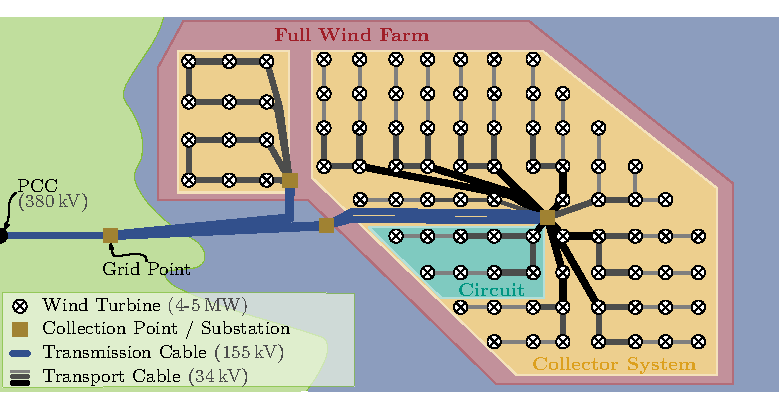
\includegraphics[page=1,scale=1]
    {windfarmplacement/figures/windparklayerCROP.pdf}
    % 
    \caption[The description of the wind farm topology.]{The wind farm topology
    typically consists of wind turbines~\tikzTurbine and
    substations~\mbox{\tikzSubstation.} The latter are connected with
    consecutive substations using the \mbox{transmission
    system\tikzTransmissionCable}. The last substation represents the \emph{grid
    point}~\tikzSubstation---building the access to the (usually)
    high-voltage~\gls{ac} power grid---building the interface to
    the~\gls{pcc}~\tikzPCC. Wind turbines forming a connected component are
    called circuit. Multiple circuits connected to a substation constitute a
    collector system. Cables interconnecting turbines and connecting turbines
    with substations are called
    \mbox{\emph{transport cables}\tikzTransportCable}. Both shown collector
    systems are the Alpha Ventus (left) and Borkum Riffgrund I (right) with~12
    (\SI{60}{\gls{mw}}) and~78 turbines (\SI{312}{\gls{mw}}),
    respectively.}
    % 
    \label{ch:wfcp:fig:topological-description}
\end{figure}
%
Wind farms are organized in a hierarchical fashion;
compare~\cref{ch:wfcp:fig:topological-description,ch:related-work:sec:wind-farm-cabling:fig:windfarm-overview}.
Turbines in a wind farm are usually grouped into \emph{circuits} representing
connected components attached to a \emph{collector point}, which represents a
substation. Circuits are combined at a substation to a local wind turbine grid
known as \emph{collector system}. Each collector system is connected to a
collector point and from there using a transmission system, possibly via
multiple substations~\parencite{online:BARD1substation}, to a unique substation
representing the \emph{grid access point} of the wind farm. The grid access
point is connected to the grid itself via the \emph{\glslongform{pcc}}
(\gls{pcc}). The wind farm network usually forms a tree network (\ie, it is
acyclic)~\cite{online:bard-offshore-1}, sometimes a cactus network (\ie, each
edge is contained in at most one cycle)~\cite{online:trianel-windpark-borkum-1}
or less commonly a meshed network~\cite{online:global-tech-1}. During the
construction of on- or offshore wind farms the cabling of turbines and
substations represents one important design question, while the location of the
wind turbines is already fixed. Within this design question, typical cabling
problem layers are the cabling of turbines within a circuit with one or multiple
cable types known as~\emph{\glslongform{cp}} (\gls{cp}), the cabling of multiple
independent circuits with one substation to a collector system, known
as~\emph{\glslongform{sp}} (\gls{sp}), and the cabling during the consideration
of multiple---not necessarily fixed---substations known
as~\emph{\glslongform{ffp}} (\gls{ffp}).
% 
\begin{figure}[t!]
    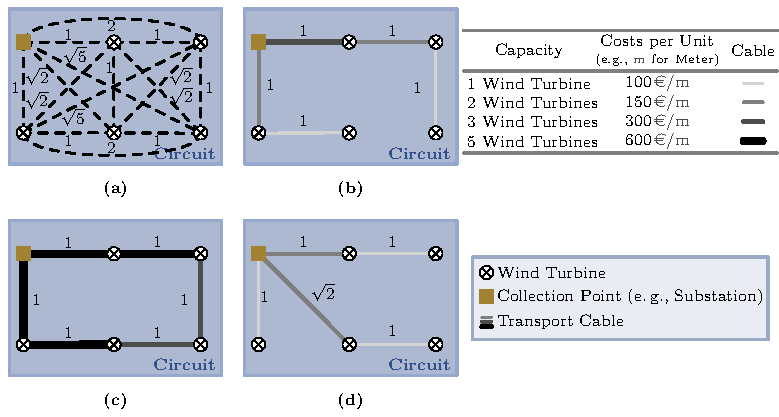
\includegraphics[page=1,scale=1]
    {windfarmplacement/figures/wind-farm-minimal-example.pdf}
    % 
    \caption[A circuit cabling example showing different cabling.]{The circuit
    of a wind farm in this small example has five wind turbines~\tikzTurbine,
    one substation~\tikzSubstation, and four possible cable
    types~\tikzTransportCable and one additional option to lay no cable type
    at all. Each cable type has a maximum capacity of power it is able to carry,
    which is shown in the table on the upper right corner. Since we assume that
    each turbine produces the same amount of power, we define the capacity in
    terms of connected turbines to a particular cable. (a) The circuit with
    its~$15$ possible cabling connections that represent a complete graph. Every
    possible connection has a certain length that is shown at each connection.
    (b) A~\acrlong{mst} (\gls{mst}) of this circuit has costs of
    about~\SI{800}{\EUR}. (c) A circuit that is cabled using a simple cycle has
    costs of about~\SI{3000}{\EUR}. (d) One best possible cabling costs
    about~\SI{662}{\EUR} and constitutes a star-shaped cabling.}
    % 
    \label{ch:wfcp:fig:wind-farm-minimal-example}
\end{figure}
% 
A simple example that describes different cabling for~\gls{sp} with their costs
is given in~\cref{ch:wfcp:fig:wind-farm-minimal-example}. It also shows that a
redundant cabling design has a significant impact on the overall costs and
that---when allowing multiple cable types---the minimum spanning tree does not
necessarily present an optimal solution to the wind farm cabling problem
(see~\cref{ch:related-work:sec:wind-farm-cabling:fig:windfarm-overview}).

We study the problem of computing a cabling in a wind farm with minimum costs
allowing different cable types and provide a model formulation using three
different levels of granularity, where the highest level represents the whole
wind farm. This is a greenfield approach for~\acrlong{tnep} (\gls{tnep}).
% 
The algorithmic issues for wind farm planning with multiple cable types are in
general~\NP-hard (see Section~\ref{ch:related-work}). To solve this~\NP-hard
problem, we propose to use~\acrlong{sa} (\gls{sa}), a well-known heuristic
approach~\parencite[pp.532ff., Section 5]{Osman1996}.
% 
We introduce a first formal hierarchical structure definition of the wind farm
problem. To evaluate our algorithm, we demonstrate on a large variety of
benchmark sets the performance of our simulated annealing algorithm. In the
following section we formalize the problem structure.
%
%%%%%%%%%%%%%%%%%%%%%%%%%%%%%%%%%%%%%%%%%%%%%%%%%%%%%%%%%%%%%%%%%%%%%%%%%%%%%%%%
%%%%%%%%%%%%%%%%%%%%%%%%%%%%%%%%%%%%%%%%%%%%%%%%%%%%%%%%%%%%%%%%%%%%%%%%%%%%%%%%
\section[A Mathematical Model for the Wind Farm Cabling Problem]{A Mathematical
Model for the \protect\linebreak{Wind Farm Cabling Problem}}
\label{ch:wfcp:sec:model}
%%%%%%%%%%%%%%%%%%%%%%%%%%%%%%%%%%%%%%%%%%%%%%%%%%%%%%%%%%%%%%%%%%%%%%%%%%%%%%%%
%
The cable layout problem for a wind farm considers mul\-ti\-ple---not
necessarily fixed---substations and different cable types.  A \emph{cable
layout} of a wind farm determines which entities are connected by cables, and
for each of them a \emph{cable type}. A \emph{valid} cable layout for a wind
farm interconnects turbines and turbines with substations in such a way that, in
the end, all turbines are connected through a path to a substation.  Further, a
valid cable layout has to support a power flow from the turbines to the
collector point in such a way that (i)~the thermal limits of the cables are
respected, and (ii)~the substation capacities are satisfied. Our goal is to find
a valid cable layout that minimizes the construction costs, which depend on the
lengths and the chosen cable types.
% 
%%%%%%%%%%%%%%%%%%%%%%%%%%%%%%%%%%%%%%%%%%%%%%%%%%%%%%%%%%%%%%%%%%%%%%%%%%%%%%%%
\paragraph{Cable Specific Definitions}
\label{ch:wfcp:sec:model:para:cable-specific-definition}
%%%%%%%%%%%%%%%%%%%%%%%%%%%%%%%%%%%%%%%%%%%%%%%%%%%%%%%%%%%%%%%%%%%%%%%%%%%%%%%%
% 
Before we model the wind farm cabling problem, we need some preliminaries.
Let~$\glssymbol{cabletypes}$ denote a set of cable types and
let~$\glssymbol{capacity}, \glssymbol{windfarmCableCost} \colon$ $
\glssymbol{cabletypes} \to \posreals \cup \{\infty\}$ denote two functions that
assign to each cable type~$\glssymbol{cabletype} \in \glssymbol{cabletypes}$ a
maximum capacity~$\capacity(\glssymbol{cabletype})$ and a
cost~$\glssymbol{windfarmCableCost}(\glssymbol{cabletype})$ per unit of length.
For~$\glssymbol{cabletype}_{1},\glssymbol{cabletype}_{2} \in
\glssymbol{cabletypes}$ we define~$\glssymbol{cabletype}_{1} <
\glssymbol{cabletype}_{2}$ if and only
if~\mbox{$\glssymbol{capacity}(\glssymbol{cabletype}_{1}) <
\glssymbol{capacity}(\glssymbol{cabletype}_{2})$}
and~$\glssymbol{windfarmCableCost}(\glssymbol{cabletype}_{1}) <
\glssymbol{windfarmCableCost}(\glssymbol{cabletype}_{2})$.  Without loss of
generality, we assume that~$<$ is a strict total ordering
on~$\glssymbol{cabletypes}$ (it never makes sense to use a more expensive cable
with same or lower capacity). We further assume that there exist two special
cable types~$\glssymbol{cabletype}_{0},
\glssymbol{cabletype}_{{\infty}} \in \glssymbol{cabletypes}$ with~$
\glssymbol{capacity}(\glssymbol{cabletype}_{0}) 
=
\glssymbol{windfarmCableCost}(\glssymbol{cabletype}_{0}) 
= 
0$ and~$
\glssymbol{capacity}(\glssymbol{cabletype}_{\infty}) 
=
\glssymbol{windfarmCableCost}(\glssymbol{cabletype}_{\infty}) 
= 
\infty
$, where the former allows to easily model connections that are not used and the
latter is used to make every instance feasible, though possibly with infinite
costs.
% 
%%%%%%%%%%%%%%%%%%%%%%%%%%%%%%%%%%%%%%%%%%%%%%%%%%%%%%%%%%%%%%%%%%%%%%%%%%%%%%%%
\paragraph{Topology and Flows}
\label{ch:wfcp:sec:model:para:topology-and-flows}
%%%%%%%%%%%%%%%%%%%%%%%%%%%%%%%%%%%%%%%%%%%%%%%%%%%%%%%%%%%%%%%%%%%%%%%%%%%%%%%%
% 
A bidirected graph is a graph~$\glssymbol{graph} = (\glssymbol{vertices},
\glssymbol{edges})$ with vertex set~$\glssymbol{vertices}$ and edge
set~$\glssymbol{edges}$ that contains each edge in both directions.  We
use~$\glssymbol{undirectededges}$ to denote the underlying undirected edge set,
and for~$\edge \in \glssymbol{edges}$ we denote by~$\undirectededge \in
\glssymbol{undirectededges}$ the underlying undirected edge, i.e.,
$\makeUndirected{(\vertexa,\vertexb)} = \makeUndirected{(\vertexb, \vertexa)} =
\{\vertexa, \vertexb\}$. A \emph{flow} on a bidirected graph~$\glssymbol{graph}
= (\glssymbol{vertices}, \glssymbol{edges})$ is a function~$\glssymbol{flow}
\colon \glssymbol{edges} \to \reals$ satisfying the skew-symmetry property~$
\glssymbol{flow}(\vertexa, \vertexb) =  -\glssymbol{flow}(\vertexb,\vertexa)$
for all~\mbox{$(\vertexa,\vertexb) \in \glssymbol{edges}$}. We denote the
\emph{net out-flow} of each vertex~$\vertexa$ in~$\glssymbol{vertices}$
as~$\glssymbol{netflow}(\vertexa)=\sum_{(\vertexa,\vertexb) \in
\glssymbol{edges}}\glssymbol{flow}(\vertexa,\vertexb)$.
% 
%%%%%%%%%%%%%%%%%%%%%%%%%%%%%%%%%%%%%%%%%%%%%%%%%%%%%%%%%%%%%%%%%%%%%%%%%%%%%%%%
\paragraph{Wind Farm Cabling Model}
\label{ch:wfcp:sec:model:para:wind-farm-cabling-model}
%%%%%%%%%%%%%%%%%%%%%%%%%%%%%%%%%%%%%%%%%%%%%%%%%%%%%%%%%%%%%%%%%%%%%%%%%%%%%%%%
% 
We are now ready to present our model of the general wind farm cabling problem
called \glscapitalform{ffp} (\gls{ffp}).  An instance of this problem is given
by a weighted, bidirected graph~$
\glssymbol{graph} 
= (
\glssymbol{vertices},
\glssymbol{edges}, 
\glssymbol{len}
)$, where the vertex set~$\glssymbol{vertices} = \glssymbol{consumers} \cup
\glssymbol{generators}$ is the union of the set~$\glssymbol{consumers}$ of
substations and the set~$\glssymbol{generators}$ of turbines, the
set~$\glssymbol{edges}$ of edges models the possible connections in the wind
farm, and~$\glssymbol{len} \colon
\glssymbol{undirectededges} \to \posreals$ defines the lengths of the
connections. Further, we are given a set~$\glssymbol{cabletypes}$ of cable types
and for each turbine~$\vertexa \in \glssymbol{generators}$ the amount~$
\glssymbol{realpowergeneration}
(\vertexa)
\in \posreals$ of power it supplies with fixed minimum, maximum, and
current power generation with~$
\glssymbol{realpowergenerationmin}(\vertexa)
= 
\glssymbol{realpowergenerationmax}(\vertexa) 
= 
\glssymbol{realpowergeneration}(\vertexa)$, respectively. In addition, there is
for each~$
\vertexc
\in
\glssymbol{consumers}$ its minimum, maximum, and current 
capacity~$
\glssymbol{realpowerdemandmin}(\vertexc),
\glssymbol{realpowerdemandmax}(\vertexc),
\glssymbol{realpowerdemand}(\vertexc) 
\in 
\posreals$. We assume that the minimum substation capacity is zero meaning~$
\glssymbol{realpowerdemandmin} \equiv 0$.
 
A solution to such an instance is a
pair~$(\glssymbol{cabletype},\glssymbol{flow})$ where~$\glssymbol{cabletype}
\colon \glssymbol{undirectededges} \to \glssymbol{cabletypes}$ is a cable
assignment and~$\glssymbol{flow}$ is a flow on~$\glssymbol{graph}$ satisfying
the~\emph{conservation of flow} and the \emph{edge capacity} constraints.  The
conservation of flow
(\crefrange{ch:wfcp:eq:total-net-flow}{ch:wfcp:eq:substation-net-flow})
describes the flow at each vertex including the production of wind turbines
(\cref{ch:wfcp:eq:turbine-net-flow}) and capacity restrictions at substations
(\cref{ch:wfcp:eq:substation-net-flow}). The capacity restrictions of
substations should be in general described by~$\sum_{(\vertexa,
\vertexb)\in\glssymbol{edges}}\max\big(0,\glssymbol{flow}
(\vertexa,\vertexb)\big)\leq\glssymbol{realpowerdemand}(\vertexb)$ for
all~$\vertexb\in\glssymbol{consumers}$. However, we assume that there is no
positive flow leaving any substation (\cref{ch:wfcp:eq:substation-net-flow}).
The edge capacity constraints (\cref{ch:wfcp:eq:capacity-constraint}) require
that the flow on each edge respects the thermal limits of the chosen cable type.
% 
%
\begin{align}
    % 
    \sum_{\vertexa\in\glssymbol{vertices}} 
    &\glssymbol{netflow}(\vertexa)  
    &=\,\,      
    & 0,
    \label{ch:wfcp:eq:total-net-flow}
    \\
    & \glssymbol{netflow}(\vertexa)  
    &=\,\,      
    &-\glssymbol{realpowergeneration}(\vertexa) %\supply_{\vertexa} 
    &\vertexa\in\glssymbol{generators},%\turbines       
    \label{ch:wfcp:eq:turbine-net-flow}
    \\
    & \glssymbol{netflow}(\vertexa)  
    & \leq\,\,   
    & \glssymbol{realpowerdemand}(\vertexa)%\demand_{\vertexa} 
    & \vertexa\in\glssymbol{consumers},%\substations
    \label{ch:wfcp:eq:substation-net-flow}
    \\
    & \fmagnitude{\glssymbol{flow}(\edge)}
    & \leq\,\,   
    & \glssymbol{capacity}(\glssymbol{cabletype}(\makeUndirected{\edge})) 
    & \edge \in \glssymbol{edges}.
    \label{ch:wfcp:eq:capacity-constraint}
    % 
\end{align}
% 
% 
We call a pair~$(\glssymbol{cabletype},\glssymbol{flow})$ satisfying these
properties \emph{valid}. The total cost~$\glssymbol{windfarmTotalcost}(
\glssymbol{cabletype},
\glssymbol{flow})$ is given
in~\cref{ch:wfcp:eq:total-cost-FFP-free-substation-positioning}.
% 
\begin{equation}
    \glssymbol{windfarmTotalcost}(\glssymbol{cabletype},\glssymbol{flow}) 
    = 
    \sum_{\makeUndirected{\edge} \in \glssymbol{undirectededges}} 
    \left(
    \glssymbol{windfarmCableCost}(\glssymbol{cabletype}(\makeUndirected{\edge}))
    \cdot
    \glssymbol{len}(\makeUndirected{\edge})
    \right).
    % 
    \label{ch:wfcp:eq:total-cost-FFP-free-substation-positioning}
\end{equation}
% 
Our goal is to find a valid pair~$(
\glssymbol{cabletype}^\star,\glssymbol{flow}^\star)$ of minimum total cost
for~\gls{ffp} with input~$
\glssymbol{network} 
= 
(\glssymbol{graph},
\glssymbol{cabletypes},
\glssymbol{capacity}, 
\glssymbol{windfarmCableCost},%\cost,
\glssymbol{realpowergeneration},%\mathbf{\supply}, 
\glssymbol{realpowerdemand}%\mathbf{\demand}
)$.
% 
% 
We denote the optimum cost of such a solution
by~$
    \opt_{\gls{ffp}}(\glssymbol{network})
    \coloneqq
    \min
    \glssymbol{windfarmTotalcost}(\glssymbol{cabletype},\glssymbol{flow})
$.
% 
\begingroup
    \begin{problem}[framed]{\glscapitalform{ffp}~$\gls{ffp}(\glssymbol{network})$}%
    Instance: & A network corresponding to the whole wind farm~$
    \glssymbol{network} 
    = 
    (\glssymbol{graph},
    \glssymbol{cabletypes},
    \glssymbol{capacity}, 
    \glssymbol{windfarmCableCost},%
    \glssymbol{realpowergeneration},%
    \glssymbol{realpowerdemand}%
    )$.
    \\
    % 
    Objective: & Find a valid pair~$(\glssymbol{cabletype},\glssymbol{flow})$
    that minimizes the total
    cost~$\glssymbol{windfarmTotalcost}(\glssymbol{cabletype},\glssymbol{flow})$
    while
    complying with~\crefrange{ch:wfcp:eq:total-net-flow}
    {ch:wfcp:eq:capacity-constraint}.
    % 
\end{problem}%
    \label{ch:wfcp:problems:wfcp-full-farm-problem}
\endgroup

We note that our model only requires~$\glssymbol{flow}$ to be a
\emph{combinatorial flow}, \ie, it satisfies Kirchhoff's current law
(\gls{kcl}), and not necessarily an \emph{electrical flow} (power flow)
satisfying also Kirchhoff's voltage law (\gls{kvl}). However, this is not a
restriction in our setting.  First of all, our heuristics mainly produce tree
networks, and it is known that in this setting every combinatorial flow is also
a power flow (see~\cref{ch:facts:thm:fvs} on 
Page~\pageref{ch:facts:thm:fvs}). While our mixed-integer linear
program can also produce network topologies that are not trees, this happens
only rarely.
% ; see Appendix~\ref{sec:examples-simulation}
% and the structure is typically such that the flows are still valid
% power flows
%
% 
\begin{figure}[tb!]
    \begin{subfigure}{.45\textwidth}
      \vspace{0.41cm}
      \setlength{\tabcolsep}{0.2em}
\aboverulesep=0ex
\belowrulesep=0ex
\arrayrulecolor{ColorTableRule}
\centering
\begin{tabular}{c|c|c}
% 
\toprule
	Cable type 
	& Capacity~$\glssymbol{capacity}$
	& Cost per unit~$\glssymbol{windfarmCableCost}$ \\
\midrule
%-------------------------------------------------------------------------------
%-------------------------------------------------------------------------------
\rowcolor{Table-Line-Marker}
%-------------------------------------------------------------------------------
	1 	& 5 		& 20 \\
%-------------------------------------------------------------------------------
%-------------------------------------------------------------------------------
	2 	& 8 		& 25 \\
%-------------------------------------------------------------------------------
%-------------------------------------------------------------------------------
\rowcolor{Table-Line-Marker}
%-------------------------------------------------------------------------------
	3 	& 12 	& 27 \\
%-------------------------------------------------------------------------------
%-------------------------------------------------------------------------------
	4 	& 15 	& 41 \\
%-------------------------------------------------------------------------------
%-------------------------------------------------------------------------------
\bottomrule
%-------------------------------------------------------------------------------
%-------------------------------------------------------------------------------
\end{tabular}
  
      \vspace{0.4cm}
      \caption{}
      \label{ch:wfcp:tbl:cabletypes}
    \end{subfigure}
    \hfill
    \begin{subfigure}{.45\textwidth}
      \hspace{0.5cm}
      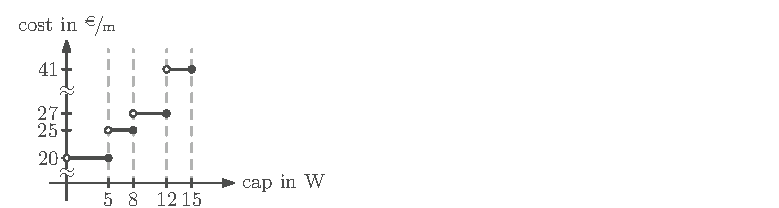
\includegraphics{windfarmplacement/figures/cable-types-stair-case-function.pdf}
      \caption{}
      \label{ch:wfcp:fig:cabletypes}
    \end{subfigure}
    % 
    \caption[An example set of cable types.]{The cable types for our experiments
    are based on~\textcite{berzan}. The cost for a cable on an edge is the
    product of the cost per length~\glssymbol{windfarmCableCost} (\eg, in
    Euro~\si{\EUR\per\metre}) and the euclidean distance (\eg, in meter~
    \si{\metre}). Note that each cable has a certain capacity~
    \glssymbol{capacity} (\eg, using real
    power in Watt~\si{\glssymbol{watt}}). (a) The cable types in tabular form.
    (b) The diagram's x-axis represents the cable capacity (\eg, in terms of
    real power in~\gls{watt}) and its y-axis represents the costs~$
    \glssymbol{windfarmCableCost}$ (\eg, in~$\si{\EUR\per\metre}$). The cable
    types in a diagram illustrate the non-convex staircase cost function. If the
    line ends with a dark filled cycle the value is included and otherwise it is
    not.}
    % 
    \label{ch:wfcp:tbl:fig:cabletypes}
\end{figure}
%  
%%%%%%%%%%%%%%%%%%%%%%%%%%%%%%%%%%%%%%%%%%%%%%%%%%%%%%%%%%%%%%%%%%%%%%%%%%%%%%%%
\paragraph{Transformation to a Minimum Cost Flow Problem}
\label{ch:wfcp:sec:model:para:transformation-to-min-cost}
%%%%%%%%%%%%%%%%%%%%%%%%%%%%%%%%%%%%%%%%%%%%%%%%%%%%%%%%%%%%%%%%%%%%%%%%%%%%%%%%
% 
In the following we transform this problem into a minimum cost flow problem on
the input graph~$\glssymbol{graph}$, but with non-convex staircase cost
functions (see~\cref{ch:wfcp:fig:cabletypes}).  For this, we first observe that, given a flow~$
\glssymbol{flow}$
on~$\glssymbol{graph}$
satisfying~\crefrange{ch:wfcp:eq:total-net-flow}{ch:wfcp:eq:substation-net-flow},
it is easy to construct a cable assignment~$\glssymbol{cabletype}$ of minimum
cost such that~$(\glssymbol{cabletype}, \glssymbol{flow})$ is valid.  Namely,
for each edge~$\makeUndirected{
\edge}\in \glssymbol{undirectededges}$, we
define~$
\glssymbol{cabletype}_{\glssymbol{flow}}(\makeUndirected{\edge}) 
= 
\min 
\{ 
\glssymbol{cabletype} \in \glssymbol{cabletypes} 
\mid 
\fmagnitude{\glssymbol{flow}(\edge)} 
\le
\glssymbol{capacity}(\glssymbol{cabletype})
\}
$, \ie, $\glssymbol{cabletype}_{\glssymbol{flow}}(\makeUndirected{\edge})$ is
the cable type with the smallest capacity (and by our assumption
on~$\glssymbol{cabletypes}$ also with the smallest cost) whose capacity is large
enough so that~\cref{ch:wfcp:eq:capacity-constraint} is satisfied
for~$\glssymbol{flow}$.  Note that the cost associated with edge~$
\makeUndirected{\edge}
=
\{\vertexa, \vertexb\}
$ then is~$
\glssymbol{windfarmCableCost}(\glssymbol{cabletype}_{\glssymbol{flow}}
(\undirectededge))
\cdot
\glssymbol{len}(\undirectededge)
$. Thus, by using for each edge~$
\edge \in \glssymbol{edges}
$ the cost function~$
\glssymbol{windfarmCableCost}_{\edge}
\colon 
\reals
\to 
\posreals$ as
% 
\begin{equation}
    % \totalcost_\edge(x) 
    \glssymbol{windfarmCableCost}_{\edge}(x)
    = 
    \min
    \{
    \glssymbol{windfarmCableCost}(\glssymbol{cabletype}) 
    \mid
    \glssymbol{cabletype} 
    \in 
    \glssymbol{cabletypes}, 
    \fmagnitude{x} 
    \le
    \glssymbol{capacity}(\glssymbol{cabletype})
    \} 
    \cdot 
    \glssymbol{len}(\edge), 
    % 
    \label{ch:wfcp:eq:totalcost-edge}
\end{equation}
% 
the problem becomes equivalent to
a minimum-cost flow problem~$
\glssymbol{network}%_{\gls{ffp}} 
= (
\glssymbol{graph},
\glssymbol{windfarmCableCost}_\edge,%\totalcost_\edge, 
\glssymbol{realpowergeneration}, %\mathbf{\supply}, 
\glssymbol{realpowerdemand} %\mathbf{\demand}
)$ on the bidirected graph~$
\glssymbol{graph} 
= (
\glssymbol{vertices},
\glssymbol{edges}
)$ where the cost of~$x$ units of flow along an edge
is~$\glssymbol{windfarmCableCost}_\edge(x)$. %\totalcost_\edge(x)
% 
An optimal solution is a flow~$\glssymbol{flow}^\star$ minimizing~$
\sum_{\edge\in\glssymbol{edges}}
\glssymbol{windfarmCableCost}_\edge(\glssymbol{flow}^\star(\edge))$. As above,
we denote the optimal cost by~$\opt_{\gls{ffp}}(\glssymbol{network})$.
% 
% 
\begingroup
    \begin{problem}[framed]{\acrlong{mcfp}~$\gls{mcfp}_{\gls{ffp}}(\glssymbol{network})$
}%
    Instance: & A flow network~$
    \glssymbol{network} 
    = (
    \glssymbol{graph},
    \glssymbol{windfarmCableCost}_\edge, 
    \glssymbol{realpowergeneration}, %\mathbf{\supply}, 
    \glssymbol{realpowerdemand} %\mathbf{\demand}
    )$. %and a cost function~$\glssymbol{windfarmCableCost}_\edge$.
    \\
    % 
    Objective: & Find a feasible flow~\glssymbol{flow} such that the sum of the
    cost over all edges~$
    \sum_{\edge\in\glssymbol{edges}}
    \glssymbol{windfarmCableCost}_\edge(\glssymbol{flow}(\edge))
    $ is minimized.
    % 
\end{problem}%
    \label{ch:wfcp:problem:wfcp-minimum-cost-flow-problem}
\endgroup

We note that, generally,~$\glssymbol{windfarmCableCost}_\edge$ forms a
stair-case function, and thus this problem is~\NP-hard~\parencite{20084889} and
that this transformation generalizes to the case where an individual set of
cable types~$\glssymbol{cabletypes}_{\makeUndirected{\edge}}$ is specified for
each edge~$\makeUndirected{\edge}\in\glssymbol{undirectededges}$.  In our
simulations we use the same set of cable types for all edges. Further, factors
such as wind strength and turbulences affect all turbines with the same maximum
power rating in the wind farm equally~\parencite{online:offshore-windfarm-db}.
Thus, a nominal power can be used to dimension the cabling and~$
\glssymbol{realpowergeneration}(\vertexa) = 1$ can be set for
all~$\vertexa\in\glssymbol{generators}$.

The optimization of the transmission system's export cables is not considered
for the~\gls{ffp}, since it is separately improvable. However, if the
substations are flexible, export cables have to be considered. We call that
problem flexible~\gls{ffp}~(\gls{fffp}) and its optimum value is denoted
by~$\opt_{\gls{fffp}}(\glssymbol{network}(k))$. Hierarchical-wise we consider
two special cases: the~\glscapitalform{sp}~(\gls{sp}) and
the~\glscapitalform{cp} (\gls{cp}) regarding the cabling layout of a single
collector system with~$\opt_{\gls{sp}}(\glssymbol{network})$ and circuit
with~$\opt_{\gls{cp}}(\glssymbol{network})$, respectively. Note that the problem
is the same, but the network changes.
%
For the wind farm cabling problem hierarchy holds that 
\[
\opt_{\gls{ffp}}(\glssymbol{network})
\leq
\sum_{\substation \in \glssymbol{consumers}} 
\opt_{\gls{sp}}(\glssymbol{network}(\substation))
\leq 
\sum_{\substation \in \glssymbol{consumers}}
\sum_{\circuit \in \naturals}
\opt_{\gls{cp}}(\glssymbol{network}(\substation, \circuit)).
\]
Note that the~\gls{cp} is already~\NP-hard~\parencite{20084889}. 
% 
In order to provide a good solution, we need a heuristic which is described in
the following section.
% 
%%%%%%%%%%%%%%%%%%%%%%%%%%%%%%%%%%%%%%%%%%%%%%%%%%%%%%%%%%%%%%%%%%%%%%%%%%%%%%%%
%%%%%%%%%%%%%%%%%%%%%%%%%%%%%%%%%%%%%%%%%%%%%%%%%%%%%%%%%%%%%%%%%%%%%%%%%%%%%%%%
\section{Simulated Annealing-based Approach}
\label{ch:wfcp:sec:simulated-annealing}
%%%%%%%%%%%%%%%%%%%%%%%%%%%%%%%%%%%%%%%%%%%%%%%%%%%%%%%%%%%%%%%%%%%%%%%%%%%%%%%%
%
%
\begin{table}[t!]
    \caption[Values of the generated benchmark data set.]{The generated
    benchmark sets for our simulations. The
    sets~$\glssymbol{network}_1 \dots \glssymbol{network}_4$ are the sets with a
    restricted edge set~$\glssymbol{edges}$ resembling realistic wind farms in
    the sense of allowed cabling. The benchmark set~$\glssymbol{network}_5$
    represents a complete graph vertex-equivalent to~$\glssymbol{network}_3$.
    The parameters~$\glssymbol{shapeAspectRatio},
    \glssymbol{generators},
    \glssymbol{consumers},
    \glssymbol{capacityTightness}, %substationCapacityTightness
    \glssymbol{substationCapacityVariance},
    \glssymbol{kNearestNeighbor}$, and~$\glssymbol{edgeInclusionValue}$
    represent the shape aspect ratio, set of turbines, set of substations,
    substation capacity tightness, substation capacity
    variance,~$\glssymbol{kNearestNeighbor}$-nearest neighbor, and value for the
    inclusion of shortcut edges~$\glssymbol{edges}'$, respectively.}
    % 
    \label{ch:wfcp:tbl:benchmark-sets}
    % 
    \footnotesize
\setlength{\tabcolsep}{0.2em}
{\renewcommand{\arraystretch}{3}}% for the vertical padding
\aboverulesep=0ex
\belowrulesep=0ex
\arrayrulecolor{ColorTableRule}
\centering
\begin{tabular}{
m{2.7cm}
|%!{\vrule width 1pt}
>{\raggedleft}m{0.4cm}
>{\raggedleft}m{0.4cm}
|
>{\raggedleft}m{0.4cm}
>{\raggedleft}m{0.7cm}%
|
>{\raggedleft}m{0.4cm}
>{\raggedleft}m{0.4cm}
|
>{\raggedleft}m{0.5cm}
>{\raggedleft}m{0.5cm}
|
>{\raggedleft}m{0.5cm}
% >{\raggedleft}m{0.4cm}
c
|
c
|
c
% >{\raggedleft}m{0.6cm}
c
|
>{\raggedleft}m{0.7cm}
c
|
c
}
\toprule
	\multirow{2}{3cm}{Benchmark Set}
		& \multicolumn{2}{c|}{$\glssymbol{shapeAspectRatio}$}
		& \multicolumn{2}{c|}{$\fmagnitude{\glssymbol{generators}}$}
		& \multicolumn{2}{c|}{$\fmagnitude{\glssymbol{consumers}}$}
		& \multicolumn{2}{c|}{$\nicefrac{\fmagnitude{\glssymbol{generators}}}
		{\fmagnitude{\glssymbol{consumers}}}$}
		& \multicolumn{2}{c|}{$\glssymbol{capacityTightness}$}
		& \multirow{2}{0.3cm}{\centering $\glssymbol{substationCapacityVariance}$}
		& \multirow{2}{0.3cm}{\centering $\glssymbol{kNearestNeighbor}$} 
		& \multirow{2}{0.3cm}{\centering $\glssymbol{edgeInclusionValue}$}
		& \multirow{2}{0.5cm}{$\fmagnitude{\glssymbol{network}_i}$}
		& run
		& \multirow{2}{0.3cm}{$\glssymbol{temperature}_0$}
	\\[-2pt]
		& \tiny $\min$ & \tiny $\max$
		& \tiny $\min$ & \tiny $\max$
		& \tiny $\min$ & \tiny $\max$
		& \tiny $\min$ & \tiny $\max$
		& \tiny $\min$ & \tiny $\max$
		& & &
		&  & \tiny$\left[\frac{\si{\minute}}
		{\glssymbol{network}_i}\right]$ &
	\\\midrule
%-------------------------------------------------------------------------------
%-------------------------------------------------------------------------------
\rowcolor{Table-Line-Marker}
%-------------------------------------------------------------------------------
	$\glssymbol{network}_1$ small/single
		& 0.7 & 1
		& 10 & 80
		& 1 & 1
		& -- & --
		& -- & --
		& --
		& 6 & 1.1
		& 500
		& 2
		& 0.01
	\\
%-------------------------------------------------------------------------------
%-------------------------------------------------------------------------------
	$\glssymbol{network}_2$ small
		& 0.7 & 1
		& 10 & 80
		& 2 & 7
		& 10 & 20
		& 0.83 & 1
		& 0
		& 6 & 1.1
		& 500
		& 2
		& 0.01
	\\
%-------------------------------------------------------------------------------
%-------------------------------------------------------------------------------
\rowcolor{Table-Line-Marker}
%-------------------------------------------------------------------------------
	$\glssymbol{network}_3$ medium
		& 0.5 & 1
		& 80 & 200
		& 4 & 10
		& 10 & 20
		& 0.83 & 1
		& 0
		& 6 & 1.1
		& \SI{1000}{}
		& 30
		& 0.01
	\\
%-------------------------------------------------------------------------------
%-------------------------------------------------------------------------------
	$\glssymbol{network}_4$ large
		& 0.4 & 1
		& 200 & \SI{1000}{}
		& 10 & 40
		& 10 & 50
		& 0.83 & 1
		& 0
		& 6 & 1.1
		& \SI{1000}{}
		& 30
		& 0.01
	\\\midrule
%-------------------------------------------------------------------------------
%-------------------------------------------------------------------------------
\rowcolor{Table-Line-Marker}
%-------------------------------------------------------------------------------
	$\glssymbol{network}_5$ medium/complete
		& 0.5 & 1
		& 80 & 200
		& 4 & 10
		& 10 & 20
		& 0.83 & 1
		& 0
		& $(\fmagnitude{\glssymbol{vertices}}-1)$ 
		& --
		& \SI{1000}{}
		& 30
		& 0.01
	\\\bottomrule
\end{tabular}

\end{table}
% 
%
The layout problem for multiple cable types is~\NP-hard~\parencite{20084889}.
Thus, this optimization problem becomes impracticable using combinatorial
methods as the problem size grows.  However, meta-heuristics such
as~\acrlong{sa}~(\gls{sa})~\parencite{Kirkpatrick83optimizationby, Cerny1985}
are promising probabilistic approaches---especially for large search
spaces---even though they do not necessarily find an optimum, but often a very
good solution. \gls{sa} is often used for optimization problems where the search
space is discrete such as the cabling problem. The Metropolis
algorithm~\cite{Metropolis1953} and the cooling schedule represent two
characteristic methods of the~\gls{sa} algorithm. The~\gls{sa} approach
calculates a finite set of solutions~$\glssymbol{solutions}$ (since the number
of iteration is finite). A solution at
time~\mbox{$\glssymbol{timestamp}\in\naturals$} is denoted
by~$\glssymbol{solution}_{\glssymbol{timestamp}}\in\glssymbol{solutions}$, where
each solution is a tuple~$
\glssymbol{solution}_{\glssymbol{timestamp}}
=
(\glssymbol{network}^{\glssymbol{timestamp}},
\glssymbol{flow}^{\glssymbol{timestamp}})
$
with a flow network~$\glssymbol{network}$ at time~$\glssymbol{timestamp}$, where
the underlying graph~$\glssymbol{graph}$ changes dependent
on~$\glssymbol{timestamp}$ denoted
by~$\glssymbol{graph}^{\glssymbol{timestamp}}=(\vertices,
\glssymbol{edges}^{\glssymbol{timestamp}})$ with
$\glssymbol{edges}^{\glssymbol{timestamp}}\subseteq\glssymbol{edges}$. By
using~\cref{ch:wfcp:eq:totalcost-edge}, we have a real-valued cost function for
our~\gls{sa} approach, which is defined in~\cref{ch:wfcp:sa:eq:totalcost-edge}.
% 
\begin{equation}
    \glssymbol{windfarmTotalcost}(\glssymbol{solution}_{\glssymbol{timestamp}})
    =
    \sum_{\edge\in\glssymbol{edges}^{\glssymbol{timestamp}}}
    \glssymbol{windfarmCableCost}_\edge(\glssymbol{flow}(\edge)). 
    % 
    \label{ch:wfcp:sa:eq:totalcost-edge}
\end{equation}
% 
We call a solution \emph{feasible} if the flow~$\glssymbol{flow}$ is feasible
and the graph~$\glssymbol{graph}^{\glssymbol{timestamp}}$ is connected. The
global optimum for problem~$\glssymbol{problems}$ (see~\cref{ch:wfcp:sec:model})
minimizing
the total cost~$\totalcost(\glssymbol{solution}^{\star})$ is a feasible
solution~$\glssymbol{solution}^{\star}=(\glssymbol{network}^\star,
\glssymbol{flow}^\star)$
with~$\glssymbol{solution}^{\star}\in\glssymbol{solutions}$ and
cost~$\opt(\glssymbol{solution}^{\star})$. For each
edge~$\undirectededge\in\glssymbol{undirectededges}$, we denote the
\emph{neighborhood}~$\glssymbol{neighbor}_{\glssymbol{graph}}(\undirectededge)$
as the set of \emph{adjacent} edges that are connected to either
endpoints~$\vertexa,\vertexb$ of~$\undirectededge =\{\vertexa, \vertexb\}$
with~$
\glssymbol{neighbor}_{\glssymbol{graph}}(\undirectededge)
\subsetneq
\glssymbol{undirectededges}
-
\{\undirectededge\}$ (an
edge~$\makeUndirected{\edgea}\in\glssymbol{neighbor}_{\glssymbol{graph}}(\makeUndirected{\edgeb})$
if and only
if~$\makeUndirected{\edgeb}\in\glssymbol{neighbor}_{\glssymbol{graph}}(\makeUndirected{\edgea})$).
We write~$\glssymbol{neighbor}(\undirectededge)$ instead
of~$\glssymbol{neighbor}_{\glssymbol{graph}}(\undirectededge)$ if the underlying
graph~$\glssymbol{graph}$ is unambiguous. In a similar fashion, we define the
neighborhood of solutions, where we denote that
solution~$\solutiona\in\glssymbol{solutions}$ is neighbor of
solution~$\solutionb\in\glssymbol{solutions}$
by~$\solutiona\in\glssymbol{solutions}(\solutionb)$. The \emph{cooling schedule}
is a non-increasing monotone
function~$\glssymbol{temperature}\colon\naturals\to(0,\infty)$,
where~$\glssymbol{temperature}(\glssymbol{timestamp})$ is the temperature at
time~$\glssymbol{timestamp}$. The cooling of an object at
time~$\glssymbol{timestamp}\in\naturals$ (\cref{ch:wfcp:sa:eq:cooling-schedule})
is also influenced by the thermal conductivity and capacity represented by the
factor~$\glssymbol{thermalConductivityCapacity}$.
% 
\begin{equation}
    \glssymbol{temperature}(\glssymbol{timestamp}+1)
    =
    (1-\glssymbol{thermalConductivityCapacity})
    \cdot
    \glssymbol{temperature}(\glssymbol{timestamp})
    % 
    \label{ch:wfcp:sa:eq:cooling-schedule}
\end{equation}
% 
It influences the
probability~$\glssymbol{probability}_{\solutiona\solutionb}\in\posreals$ of
accepting a worse solution~$\solutionb$ from~$\solutiona$. All possible
probabilities are assumed to be~$
\sum_{\solutionb\in\glssymbol{solutions}(\solutiona)}
\glssymbol{probability}_{\solutiona\solutionb}
=
1$. We introduce a \emph{dynamic cooling schedule} in the following.
In~\cref{ch:wfcp:sa:eq:dynamic-cooling-schedule}, we define
the~\emph{activity}~$\glssymbol{activity}_{\glssymbol{timestamp}}$.
% 
\begin{equation}
    \glssymbol{activity}_{\glssymbol{timestamp}+1} 
    =
    \alpha_{\mathrm{smooth}}
    \glssymbol{probability}_{\mathrm{Norm}} 
    + 
    (1-\alpha_{\mathrm{smooth}})
    \glssymbol{activity}_{\glssymbol{timestamp}},
    % 
    \label{ch:wfcp:sa:eq:dynamic-cooling-schedule}% achtung eigentlich eher eine
    % activity
\end{equation}
% 
where the initial activity~$\glssymbol{activity}_{\glssymbol{timestamp} = 0} =
1$, the impact of the current probability fluctuations and the normalized
probability are denoted by $\alpha_{\mathrm{smooth}}$ and~$$
\glssymbol{probability}_{\mathrm{Norm}}
[
\glssymbol{solution}_{\glssymbol{timestamp}+1}
\mid
\glssymbol{solution}_{\glssymbol{timestamp}+1}
\in
\glssymbol{solutions}(\glssymbol{solution}_{\glssymbol{timestamp}})
]
\approx
\exp(
\nicefrac{
        -\glssymbol{energy}
    }{
        \glssymbol{temperature}(\glssymbol{timestamp})
        \glssymbol{windfarmTotalcost}(\glssymbol{solution}_{\glssymbol{timestamp}})
    }),
$$ respectively, where~$
\glssymbol{energy}
=
\glssymbol{windfarmTotalcost}(\glssymbol{solution}_{\glssymbol{timestamp}+1})
-
\glssymbol{windfarmTotalcost}(\glssymbol{solution}_{\glssymbol{timestamp}})
$ represents the cost difference between the present and the next cost value
(often considered as energy). Thus, we adjust the cooling schedule
in~\cref{ch:wfcp:sa:eq:cooling-schedule} to a dynamic cooling schedule~$
\glssymbol{temperature}(\glssymbol{timestamp}+1)
= ( 
1 
- 
\glssymbol{activity}\glssymbol{thermalConductivityCapacity} 
)
\cdot
\glssymbol{temperature}(\glssymbol{timestamp})$.

An~\gls{sa} algorithm always starts with an initial
solution~$\glssymbol{solution}_{\glssymbol{timestamp} = 0}\in
\glssymbol{solutions}$. The set
of instances
is denoted by~$\glssymbol{instances}$. Further, we denote as an
\emph{instance}~$\glssymbol{instance}\in\glssymbol{instances}$ a sequence of
solutions starting with an arbitrary but fixed
solution~$\glssymbol{solution}_{\glssymbol{timestamp} = 0}$, where~$
\glssymbol{instance}=(\glssymbol{solution}_{\glssymbol{timestamp}},
\glssymbol{bestsolution}, \glssymbol{temperature})$,
with~$\glssymbol{bestsolution}$ representing the best feasible solution found so
far. Note that the standard~\gls{sa} approach holds only one instance. The
encoding is a representation of a solution
candidate~$\glssymbol{solution}_{\glssymbol{timestamp}}\in\glssymbol{solutions}$.
Our representation~$\glssymbol{representations}=(\glssymbol{potential},
\glssymbol{cuts})$ is a tuple representing a \emph{potential
field}~$\glssymbol{potential}\colon\glssymbol{vertices}\to\naturals$,
$\vertexa\mapsto x$ with~$x\in\{1,\dots,\fmagnitude{\gls{vertices}}\}$
representing a strict order on the set of turbines using the distance
function~$\glssymbol{len}(\{\vertexa,\substation\})$,
and \emph{edge cuts}~$\glssymbol{cuts}\subsetneq
\glssymbol{edges}$ with~$\glssymbol{graph}=\glssymbol{graph}-\glssymbol{cuts}$
representing the edges that are not considered as possible cable routes
(see~\cref{ch:wfcp:fig:sa-representation}\screen{a}). The potential field
avoids to lay cables to vertices having a smaller potential.
% 
\begin{figure}[t!]
    \centering
    % 
    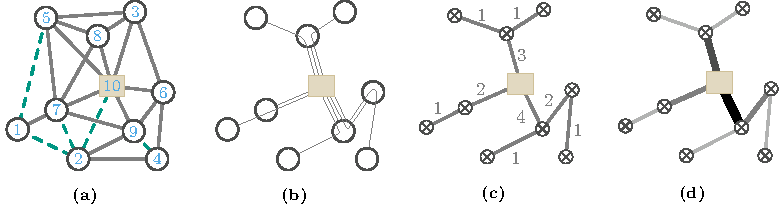
\includegraphics[page=1]{windfarmplacement/figures/representation-acm}
    % 
    \caption[The~\acrlong{sa} representation used within this work.]{Given an
    example graph~$\glssymbol{graph} = (\glssymbol{vertices},
    \glssymbol{edges})$ with vertex set~\mbox{$\glssymbol{vertices}=
    \{1,\dots,10\}$}, with a substation~$\substation\in\glssymbol{consumers}$
    represented by squares~\tikzSubstation, set of
    turbines~$\glssymbol{generators}$ represented by cycles~\tikzTurbine and set
    of edges~$\glssymbol{edges}$ represented by gray lines. (a)~The encoded
    graph~$\glssymbol{graph}$ is shown in the initial representation, where the
    cut set~$\glssymbol{cuts}$ is represented by the green dashed lines and the
    potential field~\textcolor{THETA}{\glssymbol{potential}} is represented by
    the indices in the vertices. (b)~The intermediate path representation used
    by the evaluation, where for each
    turbine~$\vertexa\in\glssymbol{generators}$ the path to the
    substation~$\vertexc\in\glssymbol{consumers}$ is shown
    with~$\fpath{}{\vertexa}{\vertexc} = \big(\vertex_0=\vertexa,
    \vertex_1, \dots,\vertex_\ell=\vertexc\big)$, where~$\{\vertex_{i},
    \vertex_{i+1}\}\in\glssymbol{undirectededges}$ for~$i=0,1,\dots,\ell$.
    (c)~The cables are labeled with the maximum cable flow, which depends on the
    number of attached turbines. (d)~The different cable types are represented
    by different diameters and colors presenting different cable types for the
    transport cables~\tikzTransportCable. Note that this is an adoption
    from~\textcite{LehMT16}.}
    % 
    \label{ch:wfcp:fig:sa-representation}
\end{figure}
% 

The set of turbines closest to substation~$\substation$ is denoted
by~$\glssymbol{generators}^{\substation}$. The
turbines~$\vertexa\in\glssymbol{generators}^{\substation}$ are ordered by
distance~$\glssymbol{len}(\{\vertexa,\substation\})$ for
each~$\substation\in\glssymbol{consumers}$ separately and their rank represents
the initial potential~$\glssymbol{potential}(\vertexa)$ and~$\glssymbol{cuts}$
is empty. To evaluate the result, the total
cost~$\glssymbol{windfarmTotalcost}(\glssymbol{solution})$ of a solution
candidate~$\glssymbol{solution}$ is calculated. However, the
representation~$\glssymbol{representations}$ does not provide a solution in the
from~$\glssymbol{solution}=(\glssymbol{network},
\glssymbol{flow})$.
Therefore, we decode~$\glssymbol{representations}$ to a path representation
(see~\cref{ch:wfcp:fig:sa-representation}\screen{b}), in which we define for each
turbine~$\vertexa\in\glssymbol{generators}^{\substation}$ a simple
path~$\fpath{}{\vertexa}{\substation} = \big(\vertex_0=\vertexa,
\vertex_1, \dots,\vertex_\ell=\substation\big)$, where~$\{\vertex_{i},
\vertex_{i+1}\}\in\glssymbol{undirectededges}$ for~$i=0,1,\dots,\ell$. The
result is used to calculate the flow by~$
\glssymbol{flow}(\vertex_i,\vertex_{i+1})
=
-\sum_{\vertex_i\in\fpath{}{\vertexa}{\substation}} 
\glssymbol{realpowergeneration}(\vertexa)
$ for all~$\vertexa\in \glssymbol{generators}$ and~$\substation\in
\glssymbol{consumers}$ (see~\cref{ch:wfcp:fig:sa-representation}\screen{c}). If
the flow~$\glssymbol{flow}$ is valid, a solution~$
\glssymbol{solution}
=(
\glssymbol{network},
\glssymbol{flow})$ exists (see~\cref{ch:wfcp:fig:sa-representation}\screen{d}).

For the wind farm planning we introduce new methods to the
\emph{diversification}---increasing the~\gls{sa} search space exploration---and
\emph{intensification}---improving a solution---phase to improve the solution
quality. In the diversification, the standard~\gls{sa} algorithm iteratively
mutates and evaluates one solution at a time. To increase the diversity of the
search space exploration, we allow multiple independent instances~$
\instancec
= (
\glssymbol{solution}^k_{\glssymbol{timestamp}},
\glssymbol{bestsolution}^{\,k},
\glssymbol{temperature}^k,
\glssymbol{thermalConductivityCapacity}^k,
\glssymbol{activity}^k
)$ of~\gls{sa} computations with~$\instancec\in\glssymbol{instances}$ each
starting with a different random seed~$k$. An \emph{activity
threshold}~$\activitythreshold$ stops a sequence of solutions once it stagnates
and falls below that activity. Further, we introduce a counter tracking the
number of iterations and resetting the instance to the best feasible
solution~$\glssymbol{bestsolution}^{\,k}$ or apply \emph{branching}
at~$\glssymbol{bestsolution}^{\,k}$. Further, we
restrict~$\fmagnitude{\glssymbol{instances}}$ to stabilize the computation time
per instance and call instances~\emph{mature} for removal, when they reach a
minimum number of mutations. Due to the fact that different solutions with
similar good energy levels provide good partial solutions, we
use~\emph{crossings} to generate new solutions based on the best parts of two
solutions. From the biological evolution, crossing provides a technique known
from evolutionary computing. We use only solutions~$\glssymbol{solution}_1,
\glssymbol{solution}_2\in\glssymbol{solutions}$ that have a high
compatibility, \ie, small minimum
cuts~$\flowvalue(\glssymbol{solution}_1,\glssymbol{solution}_2)$ among all
solutions in~\glssymbol{solutions}. To compute such a minimum cut, we use a
complete graph~$\gls{graph}_{\glssymbol{solution}_1,\glssymbol{solution}_2} = (
\gls{consumers},\binom{\fmagnitude{\gls{consumers}}}{2})$ with edge
capacities~$\gls{capacity}\colon\gls{edges}\to\naturals$, $
(\vertexa,\vertexb)\mapsto\fmagnitude{\gls{generators}^\vertexa
(\glssymbol{solution}_1)\cap\gls{generators}^\vertexb(\glssymbol{solution}_2)}$, 
with~$\vertexa,\vertexb\in\gls{consumers}$, and~$\gls{generators}^x(
\glssymbol{solution}_i)$ being the set of all turbines connected to
substation~$x\in\gls{consumers}$ of solution~$
\glssymbol{solution}_i\in\solutions$. The assignment of the potential
function~$\glssymbol{potential}$ of two solutions becomes fuzzy within the
cut region of the two partitions. Thus, we assign~$
\glssymbol{potential}(\vertex) 
= 
\ceil{
    \nicefrac{
        \left(
        \glssymbol{potential}_{\glssymbol{solution}_1}(\vertex)
        +
        \glssymbol{potential}_{\glssymbol{solution}_2}(\vertex)
        \right)
    }{2}
}$, sort the vector of potentials, and use the indices of the vector as new
potentials. For an edge~$\edge\colon(\vertexa,\vertexb)$
with~$
% 
    \vertexa,\vertexb
    \in
    \gls{generators}^x(\gls{solution}_1)
    \cap
    \gls{generators}^x(\gls{solution}_2)
% 
$ and~$x\in\gls{consumers}$, \ie both vertices are assigned to the same
substation in both solutions, we have~$\edge\in\gls{cuts}$
if~$\edge\in\gls{cuts}_{\gls{solution}_1}\cup\cuts_{
\gls{solution}_2}$. With the symmetric case, we get two new representation. 

The intensification method mutates a
representation~$\glssymbol{representations}$ by modifying either the potential
field~$\glssymbol{potential}$ or the set of cuts~$\glssymbol{cuts}$. We use
\emph{swapping} techniques to change the potential field. Either we swap the
potential of two distinct vertices~$\vertexa,\vertexb\in
\glssymbol{generators}$ randomly or we change the potential field with regard to
a potential change of a vertex~$\vertexa$. The cut-based modification is another
method using random edges. Whether we add or remove an edge to the set of
cuts~$\glssymbol{cuts}$ depends on the cardinality of~$\glssymbol{cuts}$ set
to~$\bigO(
\sqrt{\fmagnitude{\glssymbol{vertices} } })$.
%
% 
%%%%%%%%%%%%%%%%%%%%%%%%%%%%%%%%%%%%%%%%%%%%%%%%%%%%%%%%%%%%%%%%%%%%%%%%%%%%%%%%
%%%%%%%%%%%%%%%%%%%%%%%%%%%%%%%%%%%%%%%%%%%%%%%%%%%%%%%%%%%%%%%%%%%%%%%%%%%%%%%%
\section{Benchmark Generation}
\label{ch:wfcp:sec:benchmark-generator}
%%%%%%%%%%%%%%%%%%%%%%%%%%%%%%%%%%%%%%%%%%%%%%%%%%%%%%%%%%%%%%%%%%%%%%%%%%%%%%%%
%
For our thorough evaluation, we have to generate wind farms of different sizes as 
there are no published benchmark sets or generators for wind farms so far. 
In addition, current wind farms provide only a limited size and complexity. 

We introduce numerical parameters which characterize a typical wind farm. We
define the shape of a wind farm to be an ellipse described by the aspect
ratio~$\beta\in(0,1]$. The size of the shape is set such that its area is equal
to~$\fmagnitude{\glssymbol{generators}}$. Placing the turbines within this shape
is done using poisson disc
sampling~\parencite{Bridson:2007:FPD:1278780.1278807}, a random point placement
strategy in which all points are tightly placed within a minimum distance to
each other (in our case~$1$). If the new randomly generated point violates the
minimum pairwise distance, the whole farm is scaled up by an~$\epsilon>0$. The
substations are placed in the same way with a minimum pairwise distance
of~$\sqrt{\nicefrac{\fmagnitude{\glssymbol{generators}}}{\fmagnitude{
\glssymbol{consumers}}}}$.

The substation capacities are characterized by the \emph{substation capacity
tightness}~$\glssymbol{capacityTightness}$
(see~\cref{ch:wfcp:generator:eq:gamma}), which roughly states how flexible
turbines can be shifted to different substations without violating the
substation capacity~\glssymbol{realpowerdemandmax}. If the substation capacity
is tight meaning~$\glssymbol{capacityTightness} = 1$ then there is no
flexibility at all and our assumption is that it is hard to find any feasible
solution.
%
\begin{equation}
    \sum_{\vertexa\in\glssymbol{consumers}}
    \glssymbol{netflow}(\vertexa) 
    = 
    \frac{
        \sum_{\vertexb\in\glssymbol{generators}}
        \glssymbol{realpowergeneration}(\vertexb)
    }{
        \glssymbol{capacityTightness}
    }
    % 
    \label{ch:wfcp:generator:eq:gamma}
\end{equation}
%
The \emph{substation capacity variance}~$
\glssymbol{substationCapacityVariance}$ restricts the net flow at each
substation and thus, defines~$\glssymbol{realpowerdemandmin}$
and~$\glssymbol{realpowerdemandmax}$ (see~\cref{ch:wfcp:generator:eq:delta}).
%
\begin{equation}
    % 
    \glssymbol{netflow}(\vertexa)
    \in
    \left[\,
    % 
        (1-\glssymbol{substationCapacityVariance})\, 
        \frac{
            \fmagnitude{\glssymbol{generators}}
        }{
            \glssymbol{capacityTightness}\fmagnitude{\glssymbol{consumers}}
        },\;
    % 
        \glssymbol{substationCapacityVariance}\,
        \frac{
            \fmagnitude{\glssymbol{generators}}
        }{
            \glssymbol{capacityTightness}
            \fmagnitude{\glssymbol{consumers}}
        }\, 
    \right]
    \quad\forall\vertexa\in\glssymbol{consumers}
    % 
    \label{ch:wfcp:generator:eq:delta}
\end{equation}
%
We call the substation capacity~\emph{tight} if~$\glssymbol{capacityTightness}=1$ as the supply meets
the substation capacity. However, the individual substation capacities are
chosen randomly in this interval while making sure that their sum is equal
to~$\nicefrac{\sum_{\vertexb\in\glssymbol{generators}}
\glssymbol{realpowergeneration}(\vertexb)}{\glssymbol{capacityTightness}}$. Since~$\glssymbol{graph}$
is a complete graph our generator has the ability to connect all pairs of
vertices (except for export cable in the transmission system). However, we apply
a preprocessing in which we assume that direct connections over long distances
(dependent on the cable types~$\glssymbol{cabletypes}$) are uncommon, which is a
valid assumption for real world instances. Given a set of vertices we add for
each vertex~$\vertexa\in\glssymbol{vertices}$ edges to the~$k$-nearest neighbors
($k$-NN) based on the euclidean distance. In addition, we add shortcut edges
between any vertex pair having no edge in~$\glssymbol{undirectededges}$ but are
fairly near to each other, which is described
by~\cref{ch:wfcp:generator:eq:kNN}.
%
\begin{equation}
    \glssymbol{undirectededges}' 
    \coloneqq 
    \lbrace\{\vertexa,\vertexc\}
    \notin
    \glssymbol{undirectededges}
    \colon
    \glssymbol{len}(\vertexa,\vertexb)
    +
    \glssymbol{len}(\vertexb,\vertexc)
    >
    \glssymbol{edgeInclusionValue}
    \cdot
    \glssymbol{len}(\vertexa,\vertexc)
    \rbrace,
    % 
    \label{ch:wfcp:generator:eq:kNN}
\end{equation}
%
where~$\{\vertexa,\vertexb\},\{\vertexb,\vertexc\}\in
\glssymbol{undirectededges}$. We denoted the set of edges
by~$\glssymbol{undirectededges}=\glssymbol{undirectededges}\cup\glssymbol{undirectededges}'$.

Even thought the generator is able to handle distinct sets of cable types for
each edge, we generate graphs using the same set of cables for all edges, which
is standard in practice. Throughout our experiments, we use the cables
from~\textcite{berzan} obtaining their data from domain experts
(see~\cref{ch:wfcp:tbl:fig:cabletypes}).
% 
\begin{figure}[tb!]
    % 
    \begin{subfigure}{.48\textwidth}
        \scalebox{.75}{\includeplot{tau-performance-influence}}
        \vspace*{-0.465cm}\caption{}
        \label{fig:tau-performance-influence}
    \end{subfigure}\hfill%
    \begin{subfigure}{.48\textwidth}
        \scalebox{.75}{\includeplot{tightness-performance-influence}}
        \vspace*{-0.465cm}\caption{}
        \label{fig:tightness-performance-influence}
    \end{subfigure}

    \begin{subfigure}{.48\textwidth}
        \scalebox{.75}{\includeplot{cooling-schedule-SA-performance}}
        \vspace*{-0.465cm}\caption{}
        \label{fig:cooling-schedule-SA-performance}
    \end{subfigure}\hfill%
    \begin{subfigure}{.48\textwidth}
        \scalebox{.75}{\includeplot{multi-SA-instances-performance}}
        \vspace*{-0.465cm}\caption{}
        \label{fig:multi-SA-instances-performance}
    \end{subfigure}
    % 
    \caption[Comparison of our~\gls{sa} algorithm with
    the~\gls{milp}.]{Comparison of our~\gls{sa} algorithm with the~\gls{milp}.
    (a)~The value of~$\glssymbol{thermalConductivityCapacity}$ has to be chosen
    in relation to the network size. (b)~A tighter substation capacity decreases
    the performance of our~\gls{sa} approach, where
    for~$\glssymbol{capacityTightness}<0.83$ it is better. (c)~Different cooling
    schedules have different influence on the quality.
    (d)~Multi-instance~\gls{sa} performs better for networks~$\leq 450$.}
    \label{fig:SA-plots}
\end{figure}
%
%%%%%%%%%%%%%%%%%%%%%%%%%%%%%%%%%%%%%%%%%%%%%%%%%%%%%%%%%%%%%%%%%%%%%%%%%%%%%%%%
%%%%%%%%%%%%%%%%%%%%%%%%%%%%%%%%%%%%%%%%%%%%%%%%%%%%%%%%%%%%%%%%%%%%%%%%%%%%%%%%
\section{Simulations}
\label{ch:wfcp:sec:sec:simulations}
%%%%%%%%%%%%%%%%%%%%%%%%%%%%%%%%%%%%%%%%%%%%%%%%%%%%%%%%%%%%%%%%%%%%%%%%%%%%%%%%
%
In this section we run simulations of our~\gls{sa} approach and compare
instances with similar turbine to substation ratio. In an analysis we compare
the performance influence of the benchmark data on our~\gls{sa} heuristic
and~\acrlong{milp} (\gls{milp}) based on~\cref{ch:wfcp:sec:model} subject to
different criteria such as instance size~$\fmagnitude{\glssymbol{vertices}}$,
number of substations~$\fmagnitude{\glssymbol{consumers}}$ and the
\emph{substation capacity tightness} measuring the ratio of maximum supply and
demand. Our code is written in C++14, based on OGDF~2015.05~\parencite{Chi13},
Gurobi~6.5~\parencite{gurobi}, Qt 5.5; compiled with the GCC 4.8.3 with
\texttt{-O3 -march=native}. The experiment runs on a 64-\si{\bit} with four
12-core CPU of AMD~6172, clocked at~\SI{2.1}{\giga\hertz},
with~\SI{256}{\giga\byte} RAM running OpenSUSE~13.2.

In order to ensure comparability, all simulations are evaluated in single-thread
mode. The upper bound of the~\gls{milp} after~1 hour serves as our
\emph{reference solution}. For our experiments, we use the benchmark
sets~$\glssymbol{network}_\ell$ with $\ell=\{1,\dots,5\}$
(see~\cref{ch:wfcp:tbl:benchmark-sets}) generated by benchmark generator for
wind farms; see~\cref{ch:wfcp:sec:benchmark-generator}. In general we use the
benchmark sets~$\glssymbol{network}_1$ to~$\glssymbol{network}_4$, since they
work on a restricted set of edges. Note that this is already a heuristic
restriction of the solution space and thus improves the running time for both
the~\gls{milp} and the~\gls{sa} algorithm. For the small benchmark
sets~$\glssymbol{network}_1$ and~$\glssymbol{network}_2$ with shorter running
times the parameter~$\glssymbol{thermalConductivityCapacity}=10^{-5}$ represents
a good value for the cooling schedule. Whereas for the longer running
times~$\glssymbol{thermalConductivityCapacity}=10^{-6}$ results in better
solutions as the temperature is reduced more slowly. By default, the~\gls{sa}
algorithm uses a single~\gls{sa} instance, a dynamic cooling schedule and no
crossings.

For the MILP we observe different gaps after one hour running time dependent on
the wind farm size. For small networks~$\glssymbol{network}_1$
and~$\glssymbol{network}_2$, the average gap was about~$22~\%$, for
networks~$\glssymbol{network}_3$ it was \mbox{$30-31~\%$}, and
for~$\glssymbol{network}_4$ it reaches~$32~\%$. Benchmark instances with up to
13 turbines are solvable to optimality in less than an hour.

Note that the parameter~$\glssymbol{thermalConductivityCapacity}$ influences the
cooling schedule and is relevant to achieve good results
(see~\cref{fig:tau-performance-influence}). However, our~\gls{sa} algorithm
performs for~$\glssymbol{network}_1$ with one substation better than
the~\gls{milp} for~$48.2~\%$ of all benchmarks with a better average relative
cost of~$0.44~\%$. In all other cases it performs~$1.77~\%$ worse than the MILP.
Note that our~\gls{sa} algorithm takes only~$\SI{2}{\minute}$ for small networks
(see~\cref{ch:wfcp:tbl:benchmark-sets}). However, for multiple substations our
algorithm outperforms the MILP in about half of all benchmarks with a better
average relative cost of~$0.29~\%$. For the other cases it performs~$0.41~\%$
worse. The network size influences the time each iteration of the~\gls{sa}
algorithm takes,
\ie an increasing network size results in a decreasing number of iterations for
the same amount of time. For the medium and large benchmark
sets~$\glssymbol{network}_3$ with up to $200$ and~$\glssymbol{network}_4$ with
up to~$500$ turbines, both evaluated with
value~$\glssymbol{thermalConductivityCapacity} = 10^{-6}$, our~\gls{sa}
outperforms the MILP in~$7.9~\%$ of the cases due to a too short intensification
time. Thus, we increase~$\glssymbol{thermalConductivityCapacity}$ to at
least~$10^{-5}$ (see~\cref{fig:tau-performance-influence}).

The complexity of the problem can be increased by the substation capacity
tightness~$\glssymbol{capacityTightness}$
(see~\cref{fig:tightness-performance-influence}).
For~$\glssymbol{capacityTightness}=0.83$ the capacities can be up to~$20~\%$
more than the turbine supply and for~$\glssymbol{capacityTightness}=1$ there is
no variability in the number of turbines per collector system. For medium
benchmark networks and parameter
value~$\glssymbol{thermalConductivityCapacity}=8\cdot10^{-5}$ the simulations
show that the instances are more difficult to solve
for~$\glssymbol{capacityTightness}=1$, whereas more flexibility
($\glssymbol{capacityTightness}=0.83$) improves the results. Our algorithm finds
better solution for instances with~$\glssymbol{capacityTightness}<0.85$ than
the~\gls{milp}, where for~$\glssymbol{capacityTightness}>0.95$ the~\gls{milp} is
better on average.
% 
For the dynamic cooling schedule a larger value
for~$\glssymbol{thermalConductivityCapacity}$ is better, since the factor~$\mu$
drastically decreases the resulting temperature difference. By comparing the
dynamic with the standard static cooling schedule, we use
\mbox{$2^k\cdot 10^{-5}$} and~$2^k \cdot 10 ^{-7}$ with~\mbox{$k \in
\{0, 1,\dots, 7\}$}, respectively. In addition, we use for each
group~$\fmagnitude{\turbines}$ the
value~$\glssymbol{thermalConductivityCapacity}$ minimizing the average relative
performance of our algorithm. The results are shown
in~\cref{fig:cooling-schedule-SA-performance}. However, the difference between
the standard and dynamic cooling schedule is never larger than~$0.1~\%$.
In~\cref{fig:cooling-schedule-SA-performance} the dynamic cooling schedule is
more applicable for networks with up to 200 turbines, while the standard cooling
schedule is slightly better for larger networks. The dynamic cooling schedule
has a slight advantage when not
optimizing~$\glssymbol{thermalConductivityCapacity}$.

For all previous simulations, our~\gls{sa} algorithm runs one instance. Multiple
instances (see~\cref{fig:multi-SA-instances-performance}) increase the
diversification, but the total running time is distributed among all~\gls{sa}
instances in~$\instances$ resulting in a shorter intensification phase. The
results of the experiments are aggregated
using~$\glssymbol{thermalConductivityCapacity}=8\cdot 10^{-5}$ for small
and~$\glssymbol{thermalConductivityCapacity}=16\cdot 10^{-5}$ for large
instances. For small networks multiple~\gls{sa} instances are better, but for
larger instances few~\gls{sa} instances should be used. The reason is that the
diversification phase explores more of the search space with multiple~\gls{sa}
instances, but the intensification phase for large networks is too short to find
or improve good solutions.
%
%%%%%%%%%%%%%%%%%%%%%%%%%%%%%%%%%%%%%%%%%%%%%%%%%%%%%%%%%%%%%%%%%%%%%%%%%%%%%%%%
%%%%%%%%%%%%%%%%%%%%%%%%%%%%%%%%%%%%%%%%%%%%%%%%%%%%%%%%%%%%%%%%%%%%%%%%%%%%%%%%
\section{Conclusion}    
\label{ch:wfcp:sec:conclusion}
%%%%%%%%%%%%%%%%%%%%%%%%%%%%%%%%%%%%%%%%%%%%%%%%%%%%%%%%%%%%%%%%%%%%%%%%%%%%%%%%
%
In this chapter, we introduced the wind farm cabling problem and provided model
formulations for the four hierarchical layers. Since the cabling problem is
already~\NP-hard for the smallest problem layer, we introduced a novel simulated
annealing (\gls{sa}) to cope with the wind farms cabling problem. In this
context, we introduce different criteria and strategies to adapt the
standard~\gls{sa} algorithm to the cabling problem. In an extensive experimental
study, we compared our~\gls{sa} algorithm, induced by different criteria and
strategies, with the~\acrlong{milp}~(\gls{milp}) by using various benchmark data
sets, which we generated to enable comparability and to overcome the
shortcomings of the current literature. The latter used a small set of
small-sized networks, which can lead to falsifications of the results, since the
configuration of the algorithm is improved with regards to one specific data
set. We are the first that work on a great variety of benchmark data sets. In
our simulations we studied the influence of different wind farm properties on
our algorithm and~\gls{milp}. Our~\gls{sa} algorithm demonstrates excellent
performance on a variety of benchmark sets and outperforms the~\gls{milp} in
benchmark instances with up to $450$ turbines in a smaller fraction of time. It
is worth noting that we will do some future endeavors in improving our tuning
parameters and adapting the~\gls{sa} algorithm by improving and adding
strategies and tuning parameters.
